\documentclass[letterpaper, 11pt]{article}

\usepackage{amsmath, amsthm, latexsym, amssymb, graphicx, bold-extra, mathrsfs, frcursive}
\usepackage[pdftex]{color}
\usepackage[T1]{fontenc}
\usepackage{listings}
\usepackage{minted}

% Simplifies margin settings
\usepackage{geometry}
\geometry{margin=1in}

% Puts list item indicators in bold; makes flush with previous margin
\renewcommand\labelenumi{\bf\theenumi.}
\renewcommand\labelenumii{\bf\theenumii.}
% setlength\leftmargini{1.4em}
\setlength\leftmarginii{1.4em}

% Flexibility for headers and footers
\usepackage{fancyhdr}
\pagestyle{fancyplain}
\fancyhf{} %clear all header and footer fields
\lhead{\bf \small How To Write Fast Numerical Code \hspace*{\fill} Page \thepage}
\headsep 0.2in
\thispagestyle{empty}
\renewcommand{\headrulewidth}{0pt}
\renewcommand{\footrulewidth}{0pt}

\parindent 0in
\parskip 10pt
\setlength{\headheight}{20pt}

\title{ETH Zurich}

\begin{document}

%=======================================

\begin{center}
\Large \bf 263-2300-00: How To Write Fast Numerical Code

\Large \bf Assignment 1: 100 points

\large Submitted by Jinank Jain
\end{center}

\textbf{Solution 1}\\ \\
\textbf{Part a} \\
Processor Manufacturer: Intel \\
Processor Name: i7 \\
Processor Number: 3632QM \\ \\
\textbf{Part b} \\
CPU Logical Cores: 8 \\
CPU Physical Cores: 4 \\ \\ 
\textbf{Part c} \\
CPU Core frequency: 2.2 GHz \\ \\
\textbf{Part d} \\
CPU Maximum Frequency: 3.2 GHz. \\
Yes it does support Intel Turbo Boost Technology (2.0) \\ \\
\textbf{Part e} \\
Tick since my processor belongs to the family of Ivy Bridge Processor. \\ \\
\textbf{Part f-i}
\begin{table}[h!]
\centering
\label{my-label}
\begin{tabular}{|l|l|l|l|}
\hline
OpType         & Latency & Throughput & Gap \\ \hline
Addition       & 3       & 1           &  1   \\ \hline
Multiplication & 5       &  2         & 0.5    \\ \hline
rcp            &  7       &    0.5        &  2   \\ \hline
FMA            & NA      & NA         & NA  \\ \hline
\end{tabular}
\caption{Latency/Throughput/Gap for various operations}
\end{table}

\textbf{Part j} \\
Peak performance: 32 flops/cycle and 102.4 Gflops/sec
\bigskip

\textbf{Solution 2}\\ \\
\textbf{Part a} \\
Appropriate cost function would involve cost of multiplication, additions and divisions individually. One such example could be following:
\begin{equation}
\begin{aligned}
C(n) = C_{add} * N_{add} + C_{mul} * N_{mul} + C_{div} * N_{div} + C_{typecast} * N_{typecast}
\end{aligned}
\end{equation}
\textbf{Part b}
\begin{equation}
\begin{aligned}
C(n) = C_{add} *(2(n-1)+1) + C_{mul} * (6(n-1)+2) + C_{div} * (2(n-1)+2) + C_{typecast} * (2(n-1)+2) \\
\end{aligned}
\end{equation}
\begin{equation}
\begin{aligned}
C(n) = C_{add} *(2n-1) + C_{mul} * (6n-4) + C_{div} * (2n) + C_{typecast} * (2n)
\end{aligned}
\end{equation}
\begin{equation}
\begin{aligned}
C(n) = flops(n) = 12n - 5
\end{aligned}
\end{equation}

\textbf{Solution 3}\\ \\
\textbf{Part a} \\
This piece of code tries to compute matrix multiplication between two N*N matrix and store the answer in another N*N matrix \\ \\
\textbf{Part b:} \\
$C(n)$ = (adds(n), mults(n)) = ($n^3$, $n^3$) \\ \\
$C(n)$ = flops(n) = $2*n^3$ \\ \\
\textbf{Part c:}\\
Program was compiled with the following flags: \\
\texttt{-O3 -mno-abm -fno-tree-vectorize -mtune=native} \\ \\
\textbf{Part d:} \\ 
All the values that are used to plot the graph are used from RDTSC register. 
\begin{itemize}
\item Runtime Plot See Figure \ref{fig:runtime}
\item Performance Plot See Figure \ref{fig:performance} 
\item Peak performance on a single is around 8 (flops/cycle) and this value is used to plot the percentage of the peak performance See Figure \ref{fig:percentage}
\end{itemize}

\begin{figure}[h!]
    \centering
    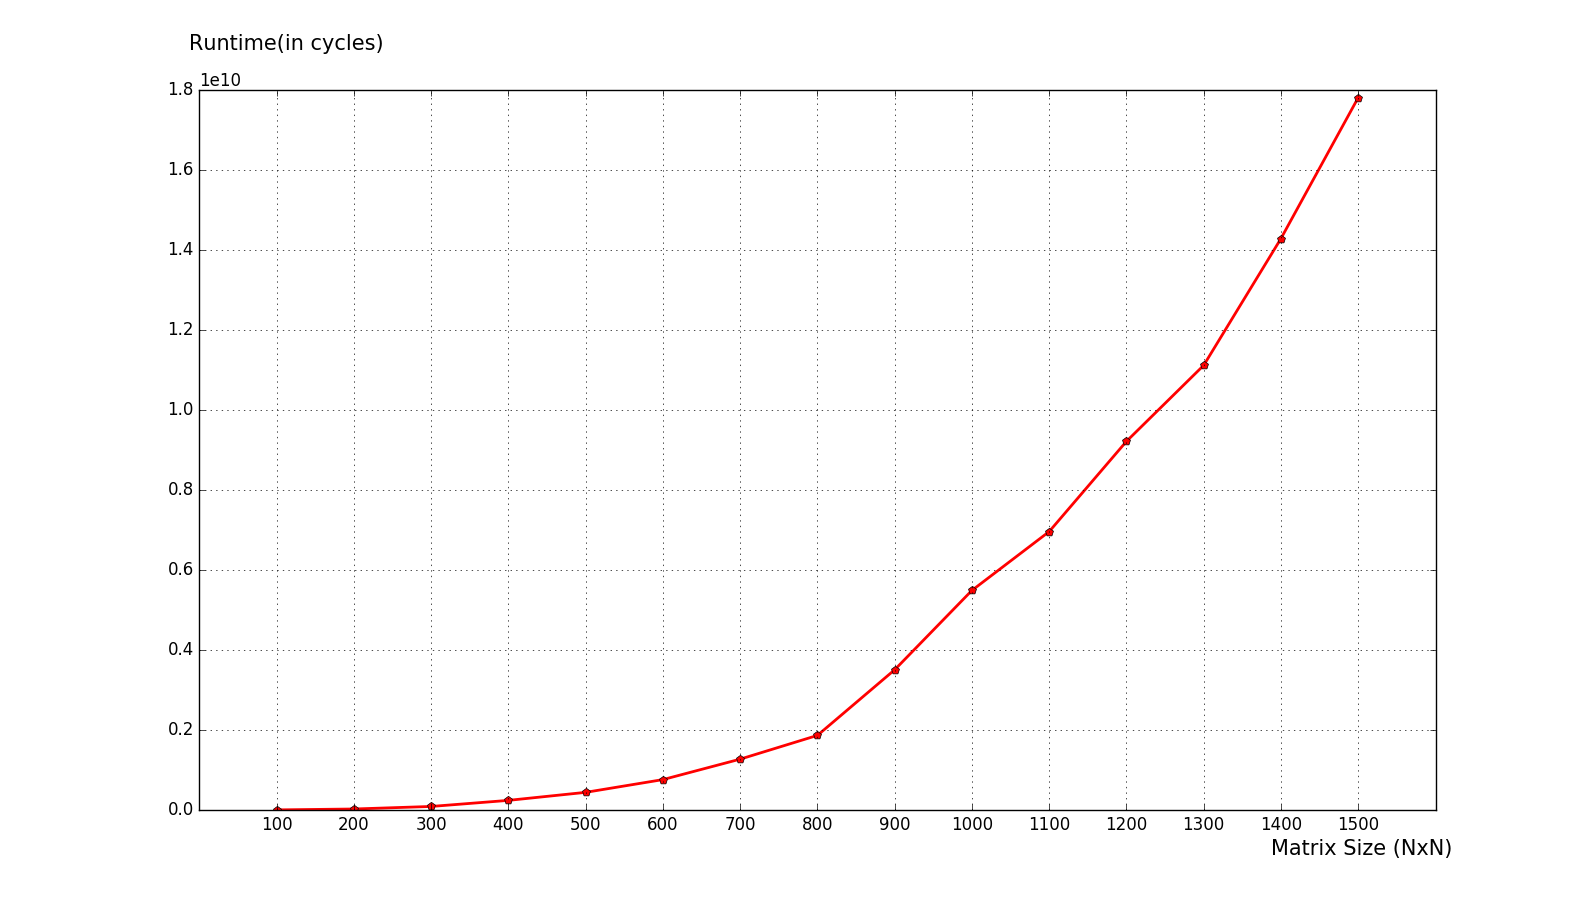
\includegraphics[width=100mm]{sol_3_1}
    \caption{Plots resulting from execution of mmm.c on a IvyBridge CPU (2.2 GHz Intel Core i7-3632QM; 32 kB L1, 256 kB L2, 6 MB L3 cache; scalar peak performance: 2 f/c). The code was compiled with gcc 6.3.1 with O3 enabled and no vectorization.}
    \label{fig:runtime}
\end{figure}

\begin{figure}[h!]
    \centering
    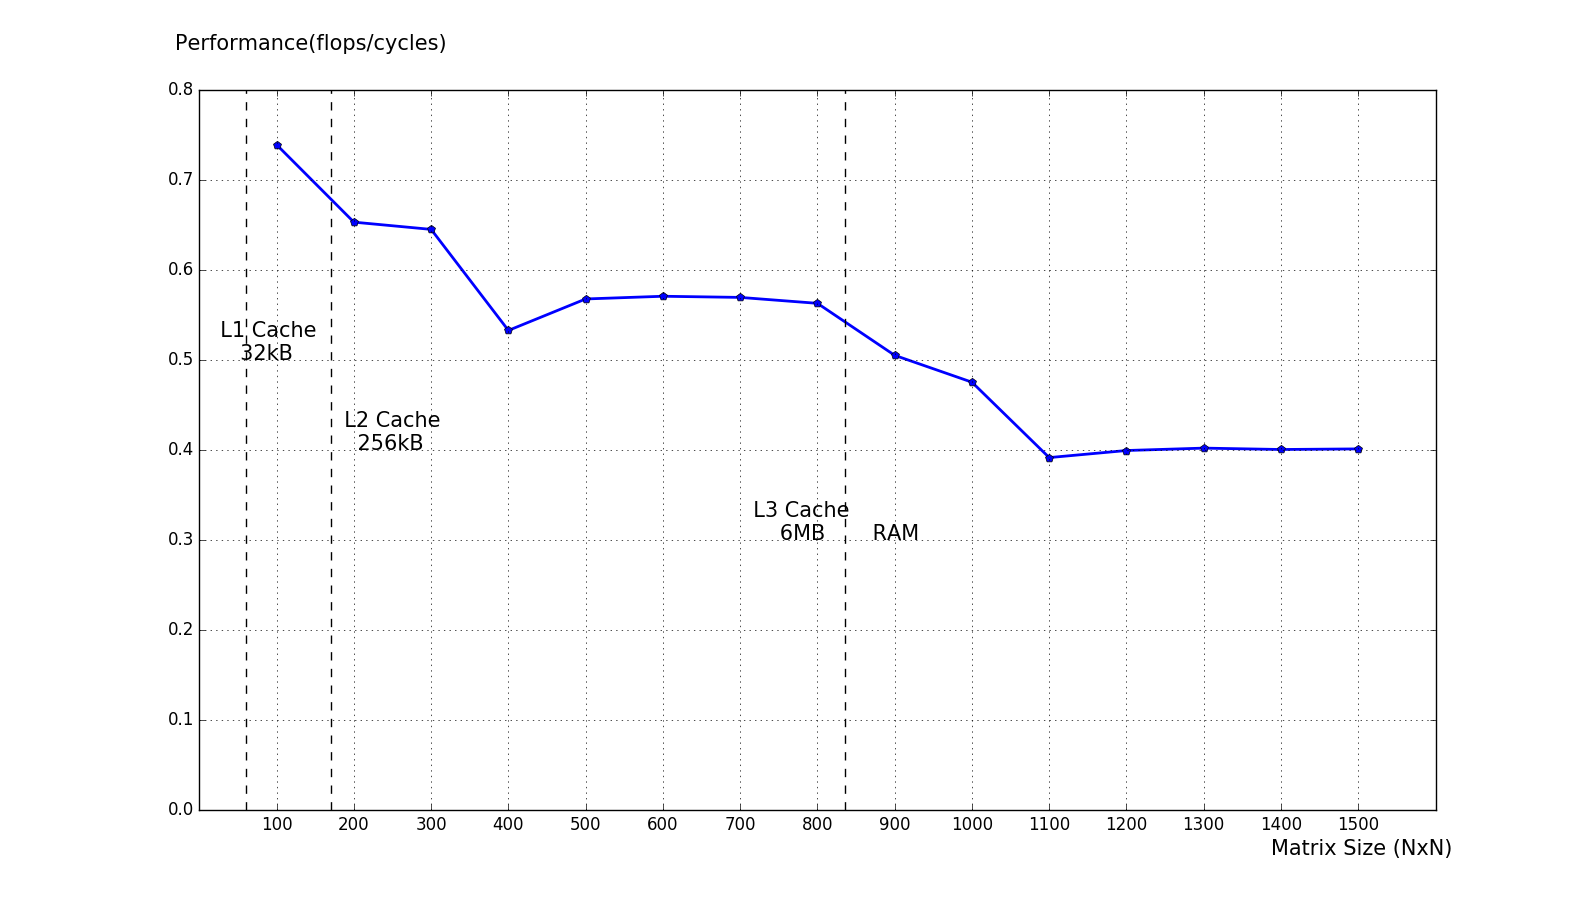
\includegraphics[width=100mm]{sol_3_2}
    \caption{Plots resulting from execution of mmm.c on a IvyBridge CPU (2.2 GHz Intel Core i7-3632QM; 32 kB L1, 256 kB L2, 6 MB L3 cache; scalar peak performance: 2 f/c). The code was compiled with gcc 6.3.1 with O3 enabled and no vectorization.}
    \label{fig:performance}
\end{figure}

\begin{figure}[h!]
    \centering
    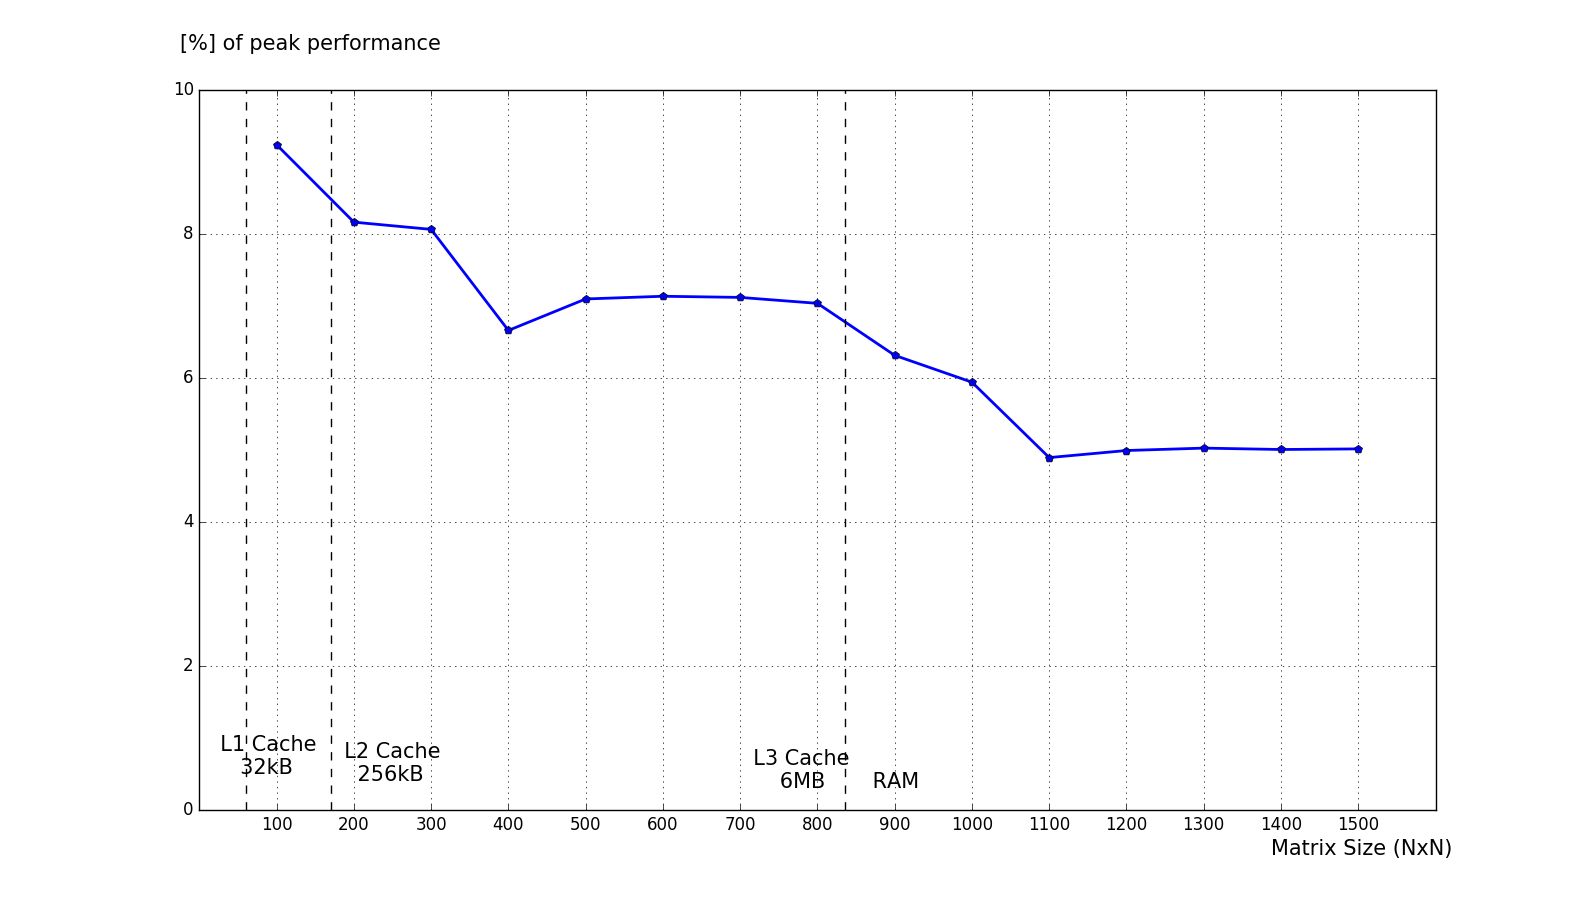
\includegraphics[width=100mm]{sol_3_3}
    \caption{Plots resulting from execution of mmm.c on a IvyBridge CPU (2.2 GHz Intel Core i7-3632QM; 32 kB L1, 256 kB L2, 6 MB L3 cache; scalar peak performance: 2 f/c). The code was compiled with gcc 4.9.3 with O3 enabled and no vectorization.}
    \label{fig:percentage}
\end{figure}
\textbf{Part e:} \\
If we look at the runtime it behaves pretty much as expected with increasing size of matrix, time required to perform the computation should increase.
The computation is compute bound however, due to dependency in the computation the peak performance cannot be achieved. Every iteration of i-loop loads matrix C, thus the performance drops whenever C does not fit in L1 (at n = 60), L2 (above n = 170) and L3 (above n = 836) cache.

\bigskip

\textbf{Solution 4}\\ \\
\textbf{Part a}
\inputminted[frame=2]{c}{sol.c}
\textbf{Part b} \\
Like in exercise 3 we used RDTSC instruction to measure the number of cycles, in this part I am using the same instruction to count the number of cycle. \\ \\
\textbf{Part c} 
Performance was measured in four different scenario:
\begin{itemize}
\item[--] Program was compiled -O3 -mno-abm -fno-tree-vectorize -mtune=native and turbo boost enabled
\item[--] Program was compiled -mno-abm -fno-tree-vectorize and turbo boost enabled
\item[--] Program was compiled -O3 -mno-abm -fno-tree-vectorize -mtune=native and turbo boost disabled
\item[--] Program was compiled -mno-abm -fno-tree-vectorize and turbo boost disabled
\end{itemize}
\begin{itemize}
\item In Figure \ref{fig:runtime_com} runtime is plotted
\item In Figure \ref{fig:performance_com} performance is plotted
\end{itemize}
\begin{figure}[h!]
    \centering
    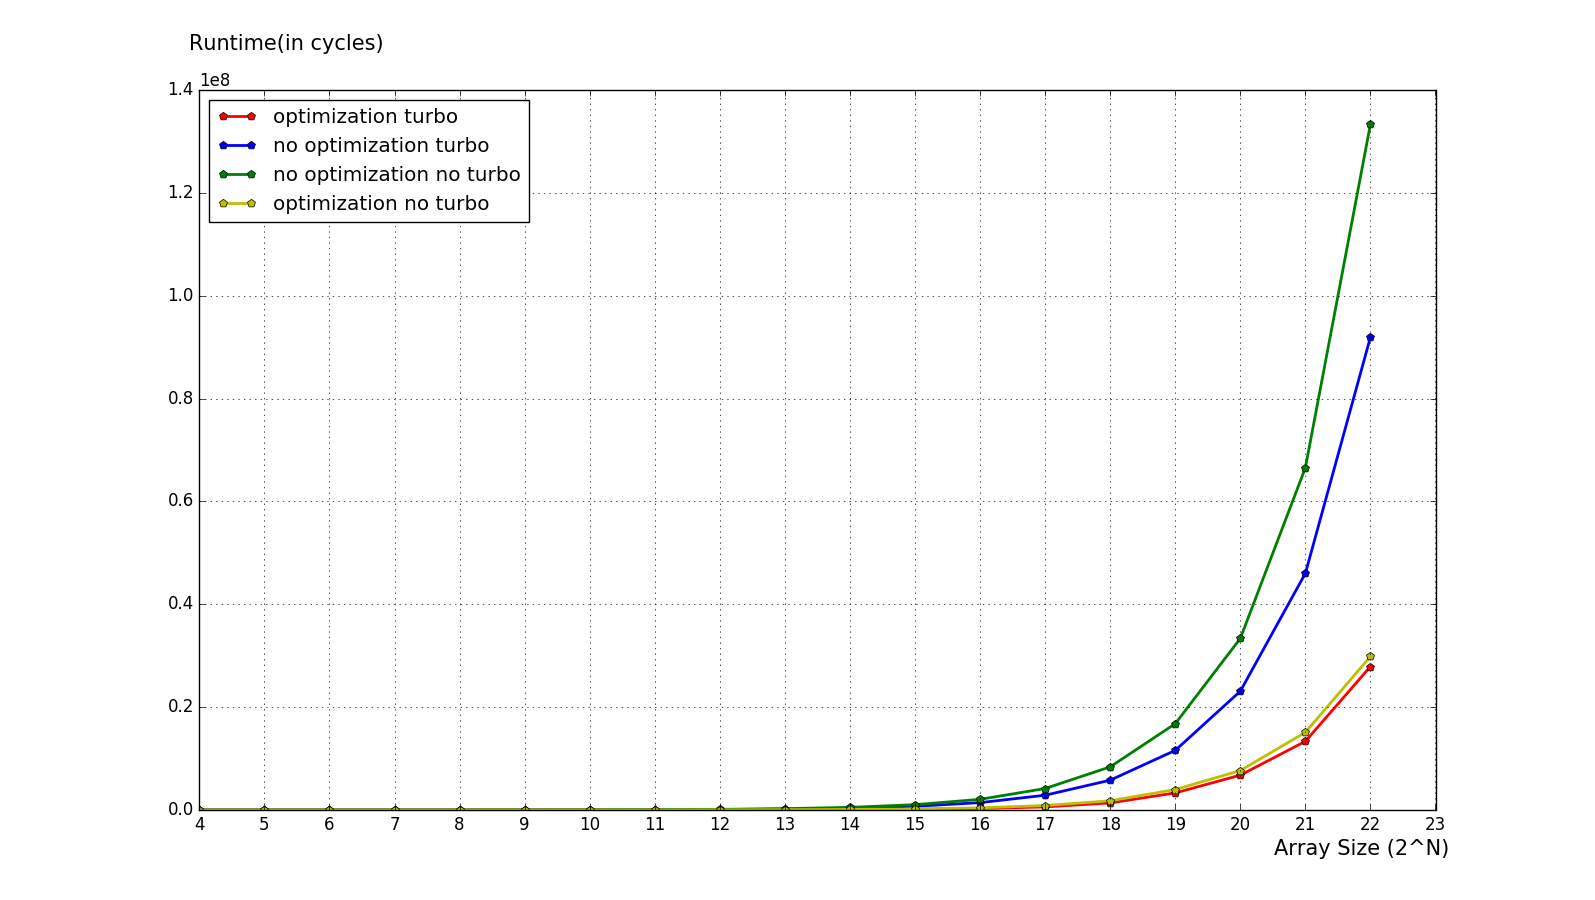
\includegraphics[width=100mm]{sol_4_1}
    \caption{Plots resulting from execution of combine.c on a IvyBridge CPU (2.2 GHz Intel Core i7-3632QM; 32 kB L1, 256 kB L2, 6 MB L3 cache; scalar peak performance: 2 f/c). The code was compiled with gcc 6.3.1}
    \label{fig:runtime_com}
\end{figure}

\begin{figure}[h!]
    \centering
    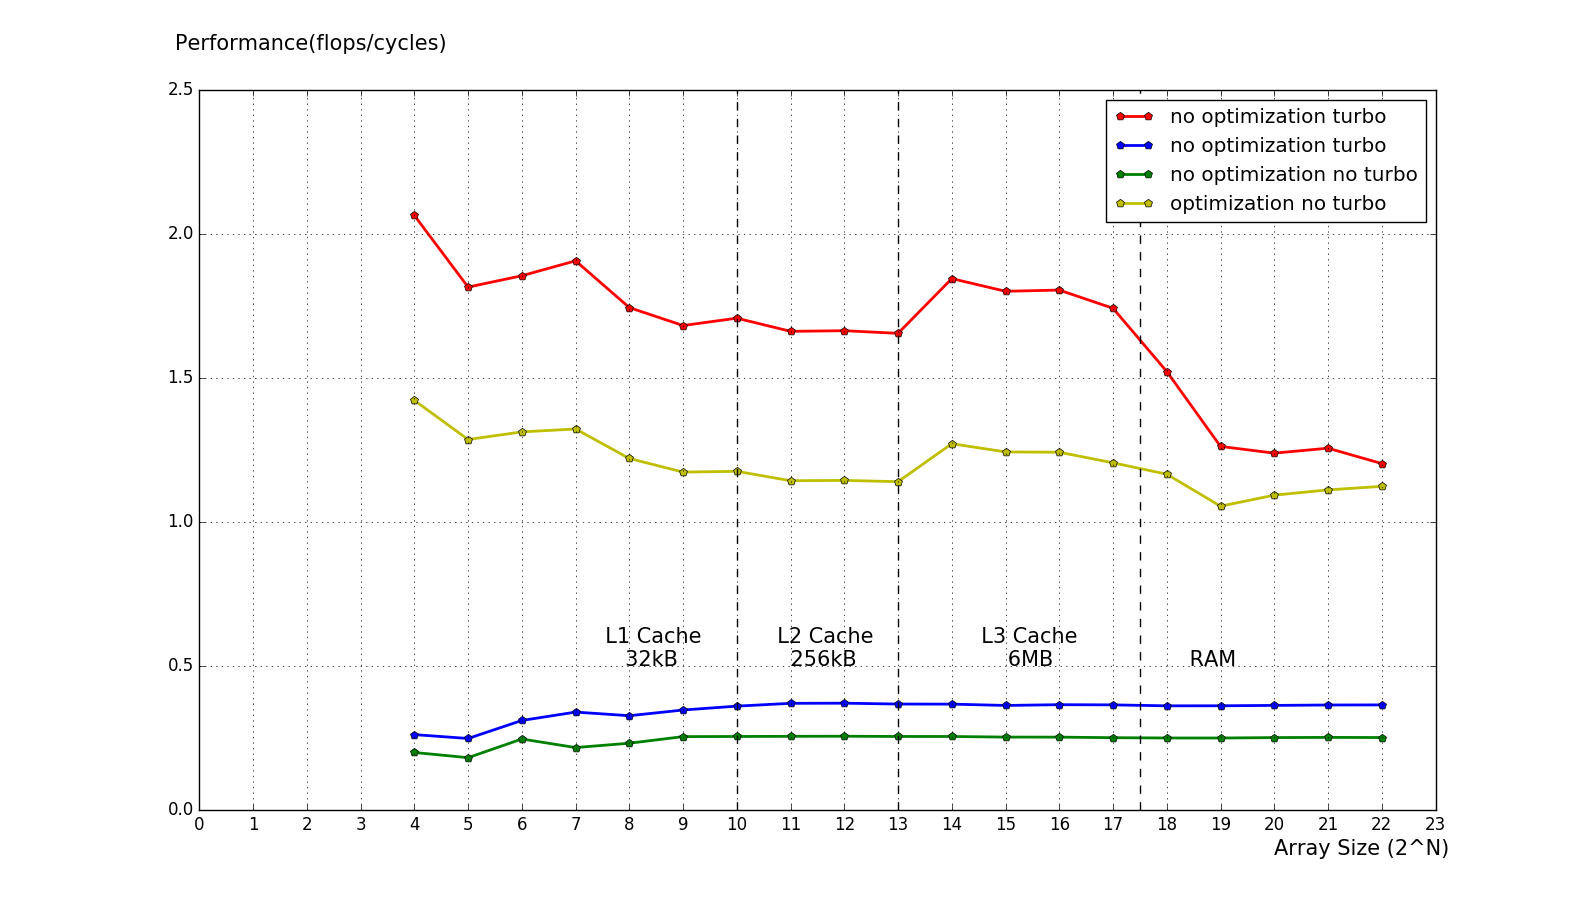
\includegraphics[width=100mm]{sol_4_2}
    \caption{Plots resulting from execution of combine.c on a IvyBridge CPU (2.2 GHz Intel Core i7-3632QM; 32 kB L1, 256 kB L2, 6 MB L3 cache; scalar peak performance: 2 f/c). The code was compiled with gcc 6.3.1}
    \label{fig:performance_com}
\end{figure}
\textbf{Part d} \\
The code is always bound by data movement 
\begin{itemize}
\item When data fits in L1, performance is bound by 1.5 f/c. On Ivy Bridge we can either issue
two loads or one load and one store at any given cycle (on port 2 and 3 of the execution
core) with an average bandwidth of 1.5 doubles per cycle. The runtime for the computation
is therefore approximately 4n doubles/1.5 doubles/c = 2.66n cycles
\item When data no more fits in L1 it goes to L2. L2 and L3 have almost the same throughput that's why in the graph we don't see any significant fluctuation in the graph in between L2 and L3.
\item When does not fit in L3 we see a significant drop in performance when we start fetching data from RAM. 
\end{itemize}
\textbf{Effect of Turboboost} \\
When turbo boost is turned on we see a significant increase in performance as it is able to operate at higher frequency. \\ \\
\textbf{Effect of Optimization Flags} \\
Optimization flags have more effect than turbo boost which is pretty much evident from the Figure 5.
\bigskip


\textbf{Solution 5}\\ \\
\textbf{Part a}
\begin{itemize}
\item \texttt{artcomp1}: 2N flops
\item \texttt{artcomp2}: N flops
\item \texttt{artcomp3}: N flops
\end{itemize}
\textbf{Part b}
\begin{itemize}
\item \texttt{artcomp1}: 
\begin{itemize}
\item Flops = 2N
\item Memory Transfers (floats) $\geq$ 2N
\item Read (bytes) $\geq$ 8N
\item Operational Intensity I(N)  $\leq \frac{1}{4}$ 
\end{itemize}
\item \texttt{artcomp2}: 
\begin{itemize}
\item Flops = N
\item Memory Transfers (floats) $\geq$ 2N
\item Read (bytes) $\geq$ 8N
\item Operational Intensity I(N)  $\leq \frac{1}{8}$ 
\end{itemize}
\item \texttt{artcomp3}: 
\begin{itemize}
\item Flops = N
\item Memory Transfers (floats) $\geq$ 2N + 2/3N
\item Read (bytes) $\geq$ 8N + 8/3 N
\item Operational Intensity I(N)  $\leq \frac{3}{32}$ 
\end{itemize}
\end{itemize}
\textbf{Part c} \\
\textbf{i}
\begin{itemize}
\item \texttt{artcomp1}:  N/2
\item \texttt{artcomp2}:  N
\item \texttt{artcomp3}:  2N/3
\end{itemize}
\textbf{ii}
\begin{itemize}
\item Order L1, L2, L3, RAM
\item \texttt{artcomp1}:  N/4, N/4, N/2, N
\item \texttt{artcomp2}:  N/4, N/8, N/4, N/2 
\item \texttt{artcomp3}:  N/4, 5N/24, 5N/12, 5N/6
\end{itemize}
\bigskip

\clearpage

%=======================================

\end{document}